\documentclass[a4paper,12pt]{article}

\usepackage[utf8]{inputenc}
\usepackage[T1]{fontenc}
\usepackage[portuguese]{babel}
\usepackage{graphicx}
\usepackage{amsmath}
\usepackage{geometry}
\usepackage{float}
\usepackage{tocloft}
\usepackage{verbatim}
\usepackage{amssymb}
\usepackage{listings}
\usepackage{xcolor}
\usepackage{booktabs}
\usepackage{float}

\lstdefinestyle{python}{
    language=Python,
    backgroundcolor=\color{gray!8},
    basicstyle=\ttfamily\small,
    keywordstyle=\color[HTML]{7F77DD}\bfseries,
    stringstyle=\color[HTML]{D85A30},
    commentstyle=\color[HTML]{888780}\itshape,
    numberstyle=\tiny\color{gray},
    numbers=left,
    numbersep=10pt,
    frame=single,
    framerule=0.4pt,
    rulecolor=\color{gray!40},
    frameround=tttt,
    breaklines=true,
    showstringspaces=false,
    tabsize=4,
    xleftmargin=12pt,
    xrightmargin=4pt,
    aboveskip=8pt,
    belowskip=8pt,
}

\renewcommand{\cftpartpresnum}{Parte\ }
\setlength{\parindent}{0pt}
\geometry{margin=2.5cm}

\addto\captionsportuguese{\renewcommand{\contentsname}{Índice Geral}}
\usepackage[hidelinks]{hyperref}
\setcounter{tocdepth}{2}

\begin{document}

% Capa
\begin{titlepage}       
    \centering
    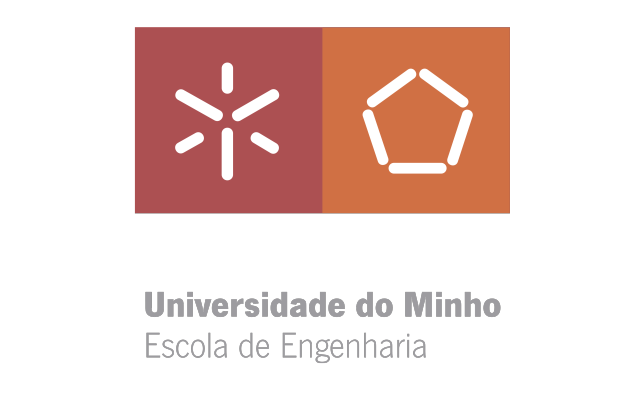
\includegraphics[width=0.5\textwidth]{imagens/LogotipoUM.png}

    \centering
    \vspace*{5cm}        
    {\Huge \textbf{Relatório Trabalho Prático Nº2 (PL32)}\par}
    \vspace{2cm}
    {\Large 
        Tomé Francisco Amorim Moreira - a111907 \\[0.3cm]
        Miguel Pedro Ribeiro Correia - a111773 \\[0.3cm]
        José Pedro Fernandes da Costa - a109807
    \par}
    \vspace*{4cm}
    {\large \today\par}
\end{titlepage}

\tableofcontents
\newpage

\section{Arquitetura do sniffer}

O sniffer desenvolvido segue uma arquitetura modular, onde cada componente tem uma responsabilidade bem definida. Esta abordagem facilita a manutenção, extensão e organização do código.

\subsection{Visão Geral}

O sistema é composto por vários módulos principais:

\begin{itemize}
    \item \textbf{main.py} – ponto de entrada da aplicação
    \item \textbf{sniffer.py} – captura e processamento de pacotes
    \item \textbf{parser.py} – extração de informação dos pacotes
    \item \textbf{stats.py} – cálculo de estatísticas globais
    \item \textbf{formatter.py} – formatação da saída
    \item \textbf{analysis.py} – modo interativo de análise
    \item \textbf{handlers/} – análise detalhada por protocolo
    \item \textbf{filters.py} – filtragem de pacotes
\end{itemize}

\subsection{Fluxo de Execução}

A execução inicia-se no módulo \texttt{main.py}, onde são processados os argumentos da linha de comandos (interface, modo de execução, ficheiro de saída e nível de verbosidade).

De seguida, é invocada a função \texttt{start\_sniffing()}, responsável por iniciar a captura de pacotes através da biblioteca Scapy.

Cada pacote capturado segue o seguinte fluxo:

\begin{enumerate}
    \item Captura do pacote (\texttt{sniffer.py})
    \item Parsing e extração de informação (\texttt{parser.py})
    \item Atualização de estatísticas globais (\texttt{stats.py})
    \item Encaminhamento para handlers específicos por protocolo
    \item Formatação da saída (\texttt{formatter.py})
    \item Impressão ou escrita em ficheiro
\end{enumerate}

\subsection{Módulo de Captura (sniffer.py)}

O módulo \texttt{sniffer.py} é responsável por:

\begin{itemize}
    \item Capturar pacotes em tempo real usando \texttt{sniff()}
    \item Manter uma lista global de pacotes capturados
    \item Invocar o parser para extrair informação relevante
    \item Encaminhar pacotes para handlers específicos (ICMP, TCP, ARP, DHCP, WiFi, etc.)
\end{itemize}

Este módulo funciona como o núcleo do sistema, coordenando os restantes componentes.

\subsection{Parser de Pacotes (parser.py)}

O \texttt{parser.py} extrai informação estruturada de cada pacote e converte-a numa instância da classe \texttt{PacketInfo}.

As principais responsabilidades incluem:

\begin{itemize}
    \item Identificação das camadas (rede, transporte, aplicação)
    \item Determinação do protocolo principal
    \item Extração de endereços MAC e IP
    \item Definição de um resumo textual do pacote
\end{itemize}

\subsection{Modelo de Dados (models.py)}

A estrutura \texttt{PacketInfo} representa cada pacote capturado e contém:

\begin{itemize}
    \item Timestamp
    \item Interface
    \item Protocolo principal
    \item Endereços MAC e IP
    \item Tamanho do pacote
    \item Resumo descritivo
\end{itemize}

Esta abstração permite desacoplar o parsing da análise.

\subsection{Estatísticas (stats.py)}

O módulo \texttt{stats.py} mantém estatísticas globais da captura, incluindo:

\begin{itemize}
    \item Número total de pacotes
    \item Volume total de tráfego
    \item Distribuição por protocolo
    \item Taxa média de transferência
\end{itemize}

As estatísticas são atualizadas em tempo real e apresentadas no final da captura.

\subsection{Handlers por Protocolo}

Os handlers, organizados na pasta \texttt{handlers/}, são responsáveis pela análise detalhada de cada protocolo identificado durante a captura. Cada handler implementa lógica específica e mantém estruturas de dados próprias para suportar análise posterior.

Ao contrário de uma simples inspeção de pacotes, estes módulos permitem reconstruir interações e extrair métricas relevantes da comunicação de rede.

\subsubsection*{Exemplos de Análise Implementada}

\begin{itemize}

\item \textbf{ICMP}  
Emparelhamento de mensagens \textit{Echo Request} e \textit{Echo Reply}, permitindo calcular o RTT (Round-Trip Time) entre dois hosts.  
São mantidas tabelas de pedidos pendentes e listas de pares completos com estatísticas associadas (mínimo, máximo e média).

\item \textbf{ARP}  
Reconstrução de pares \textit{request/reply}, identificação de pacotes \textit{gratuitous ARP} e cálculo do tempo de resposta entre pedidos e respostas.  
Permite observar resolução de endereços IP para MAC dentro da rede local.

\item \textbf{TCP}  
Análise do processo de estabelecimento de ligações TCP através do \textit{three-way handshake} (SYN, SYN-ACK, ACK).  
São identificadas conexões completas, calculado o RTT inicial e registados eventos de término (FIN) ou interrupção (RST).

\item \textbf{DHCP}  
Reconstrução de transações completas com base no identificador XID.  
Permite acompanhar as fases do protocolo (Discover, Offer, Request, ACK) e medir o tempo total de atribuição de endereço IP.

\item \textbf{IPv4}  
Deteção e análise de fragmentação IP, agrupando fragmentos por identificador.  
São apresentados offsets, tamanhos, tempos relativos de chegada e verificado se o datagrama foi completamente recebido.

\item \textbf{WiFi (IEEE 802.11)}  
Análise de frames de gestão, controlo e dados.  
Permite identificar redes ativas (beacons), dispositivos mais ativos e padrões de utilização (ex: scanning vs tráfego normal).

\end{itemize}

Cada handler mantém estruturas internas (tabelas, listas e estatísticas) que permitem uma análise posterior mais aprofundada no modo interativo.

\subsection{Formatação (formatter.py)}

Este módulo é responsável por apresentar os dados ao utilizador em dois formatos:

\begin{itemize}
    \item \textbf{Verbose} – informação detalhada
    \item \textbf{Compact} – formato resumido
\end{itemize}

\subsection{Modo de Análise (analysis.py)}

Após a fase de captura, o sistema entra num modo interativo que permite ao utilizador explorar os dados recolhidos.

Este modo funciona como uma interface de linha de comandos onde é possível executar diferentes tipos de análise sobre os pacotes armazenados.

\subsubsection*{Comandos Disponíveis}

\begin{itemize}

\item \textbf{icmp}  
Apresenta pares de mensagens ICMP (Echo Request/Reply) com cálculo de RTT.

\item \textbf{arp}  
Mostra pares de pedidos e respostas ARP, permitindo observar a resolução de endereços na rede.

\item \textbf{tcp}  
Lista conexões TCP estabelecidas, incluindo endereços, portas e RTT do handshake.

\item \textbf{dhcp}  
Apresenta fluxos de transações DHCP organizados por XID, incluindo tempos relativos entre mensagens.

\item \textbf{ipv4}  
Exibe informação detalhada sobre pacotes IPv4 (flags, TTL, tamanho, protocolo).

\item \textbf{fragments ipv4}  
Mostra grupos de fragmentos IP, permitindo analisar fragmentação e reconstrução de datagramas.

\item \textbf{wifi}  
Apresenta análise de tráfego WiFi, incluindo dispositivos ativos e redes detetadas.

\end{itemize}

\subsubsection*{Comandos de Estatísticas}

\begin{itemize}

\item \textbf{status icmp} – estatísticas de RTT e contagem de pedidos/respostas  
\item \textbf{status arp} – distribuição de pedidos, respostas e ARP gratuitous  
\item \textbf{status tcp} – contagem de eventos TCP (SYN, ACK, FIN, RST) e conexões estabelecidas  
\item \textbf{status wifi} – distribuição de tipos de frames e atividade na rede sem fios  

\end{itemize}

\subsubsection*{Filtragem de Pacotes}

O modo de análise permite ainda aplicar filtros sobre os pacotes capturados:

\begin{itemize}

\item \textbf{filter ip <endereco>} – filtra pacotes por endereço IP  
\item \textbf{filter mac <endereco>} – filtra por endereço MAC  
\item \textbf{filter proto <protocolo>} – filtra por protocolo (ex: TCP, ICMP, ARP)

\end{itemize}

\subsection{Filtragem (filters.py)}

Permite filtrar pacotes com base em:

\begin{itemize}
    \item Endereço IP
    \item Endereço MAC
    \item Protocolo
\end{itemize}

\subsection{Conclusão}

A arquitetura modular adotada permite separar claramente as responsabilidades entre captura, processamento, análise e apresentação. 
Esta abordagem facilita a extensibilidade do sistema, permitindo adicionar novos protocolos ou funcionalidades com impacto reduzido no restante código.


\section{Catalogação e Análise de Protocolos}
 
O \textit{packet sniffer} desenvolvido utiliza a biblioteca Scapy para capturar e dissecar pacotes de rede. 
A identificação dos protocolos é feita através das camadas presentes em cada pacote, sendo o handler invocado conforme o tipo detetado.
 
\subsection{ICMP — Internet Control Message Protocol}
 
\subsubsection{Identificação e tipos catalogados}
 
O protocolo ICMP é identificado pela presença da camada \texttt{ICMP} no pacote. O handler analisa o campo \texttt{icmp.type} para distinguir dois tipos de mensagem:
 
\begin{itemize}
    \item \textbf{Echo Request} (\texttt{type = 8}) — pedido de ping enviado pelo host;
    \item \textbf{Echo Reply} (\texttt{type = 0}) — resposta ao pedido, enviada pelo destino.
\end{itemize}
 
\subsubsection{Estruturas de dados}
 
A análise recorre a três estruturas principais:
 
\begin{itemize}
    \item \texttt{icmp\_table} — dicionário que armazena os requests pendentes, indexado pela tupla \texttt{(src\_ip, dst\_ip, icmp.id, icmp.seq)};
    \item \texttt{icmp\_pairs} — lista de pares completos (request + reply) com o RTT calculado;
    \item \texttt{icmp\_stats} — contadores globais de requests, replies e lista de RTTs.
\end{itemize}
 
\subsubsection{Análise e cálculo do RTT}
 
Quando um Echo Request é recebido, é registado em \texttt{icmp\_table} com a sua chave identificadora. Ao chegar um Echo Reply, a chave é invertida (sentido oposto do tráfego) e procurada nos pedidos pendentes:
 
\vspace{0.5em}

\begin{lstlisting}[style=python]
if icmp.type == 8:                          # Echo Request
    icmp_table[key] = info
 
elif icmp.type == 0:                        # Echo Reply
    reverse_key = (dst_ip, src_ip, id, seq)
    if reverse_key in icmp_table:
        rtt_ms = (info.timestamp - request.timestamp) * 1000
        icmp_pairs.append({ ..., "rtt": rtt_ms })
\end{lstlisting}
 
O RTT é obtido pela diferença entre os timestamps de captura do reply e do request correspondente, convertida para milissegundos.

\subsection{TCP — Transmission Control Protocol}
 
\subsubsection{Identificação e flags catalogadas}
 
O TCP é identificado pela camada \texttt{TCP} do pacote. A análise baseia-se no campo \texttt{tcp.flags}, que reflete o estado de cada segmento:
 
\begin{table}[H]
\centering
\begin{tabular}{lll}
\toprule
\textbf{Flag} & \textbf{Significado} & \textbf{Ação} \\
\midrule
\texttt{"S"}          & SYN     & Regista novo flow em \texttt{tcp\_flows} \\
\texttt{"SA"}         & SYN-ACK & Associa ao flow com chave invertida \\
\texttt{"A"}          & ACK     & Finaliza handshake; calcula RTT \\
\texttt{"F"} in flags & FIN     & Encerramento normal; remove flow \\
\texttt{"R"} in flags & RST     & Encerramento forçado; remove flow \\
\bottomrule
\end{tabular}
\caption{Flags TCP catalogadas pelo sniffer}
\end{table}
 
\subsubsection{Estruturas de dados}
 
A análise TCP recorre a três estruturas principais:
 
\begin{itemize}
    \item \texttt{tcp\_flows} — dicionário que armazena ligações em progresso (handshake incompleto), indexado pela tupla \texttt{(src\_ip, sport, dst\_ip, dport)};
    \item \texttt{tcp\_connections} — lista de ligações completamente estabelecidas, com RTT calculado;
    \item \texttt{tcp\_stats} — contadores globais por flag (SYN, SYN-ACK, ACK, FIN, RST) e lista de RTTs.
\end{itemize}


\subsubsection{Reconstrução do three-way handshake}
 
O sniffer reconstrói o handshake TCP estado a estado, usando \texttt{tcp\_flows} como estado intermédio indexado por \texttt{(src\_ip, sport, dst\_ip, dport)}:
 
\vspace{0.5em}

\begin{lstlisting}[style=python]
if flags == "S":                                     # SYN
    tcp_flows[key] = {"syn": info}
 
elif flags == "SA":                                  # SYN-ACK
    if reverse_key in tcp_flows:
        tcp_flows[reverse_key]["syn_ack"] = info
 
elif flags == "A" and "syn_ack" in tcp_flows[key]:  # ACK
    rtt_ms = (syn_ack.timestamp - syn.timestamp) * 1000
    tcp_connections.append({ ..., "rtt": rtt_ms })
\end{lstlisting}
 
O RTT medido corresponde ao intervalo entre o SYN e o SYN-ACK, representando a latência de resposta do servidor.
Os segmentos FIN e RST apenas removem o flow dos pendentes, sem contribuir para métricas.

\subsection{ARP — Address Resolution Protocol}

\subsubsection{Identificação e tipos catalogados}

O protocolo ARP é identificado pela presença da camada \texttt{ARP} no pacote.  
A distinção entre tipos de mensagem é feita através do campo \texttt{arp.op}:

\begin{itemize}
    \item \textbf{Request} (\texttt{op = 1}) — pedido de resolução de endereço (``quem tem este IP?'');
    \item \textbf{Reply} (\texttt{op = 2}) — resposta contendo o endereço MAC associado;
    \item \textbf{Gratuitous} (\texttt{psrc == pdst}) — anúncio espontâneo de mapeamento IP–MAC.
\end{itemize}

Os pacotes ARP Gratuitous não são considerados no emparelhamento request/reply, sendo apenas contabilizados em estatísticas globais.

\subsubsection{Semântica dos campos \texttt{psrc} e \texttt{pdst}}

Ao contrário de ICMP e TCP, o ARP opera ao nível da \textit{link layer}, utilizando uma semântica própria para endereços IP:

\begin{itemize}
    \item \texttt{psrc} — IP do emissor do pacote;
    \item \texttt{pdst} — IP alvo cuja resolução é pretendida.
\end{itemize}

Num ARP Request, \texttt{psrc} corresponde ao cliente e \texttt{pdst} ao destino procurado.  
Na resposta (ARP Reply), estes valores surgem invertidos, permitindo a correlação direta entre mensagens.

\subsubsection{Estruturas de dados}

A análise ARP recorre a três estruturas principais:

\begin{itemize}
    \item \texttt{arp\_table} — dicionário que armazena requests pendentes, indexado pela tupla \texttt{(psrc, pdst)};
    \item \texttt{arp\_pairs} — lista de pares completos (request + reply) com RTT associado;
    \item \texttt{arp\_stats} — contadores globais (requests, replies, gratuitous) e lista de RTTs.
\end{itemize}

\subsubsection{Emparelhamento e cálculo do RTT}

O handler ARP segue uma lógica semelhante à do ICMP, baseada no armazenamento temporário de requests e posterior correspondência com replies.

\vspace{0.5em}

\begin{lstlisting}[style=python]
if arp.op == 1:                         # ARP Request
    arp_stats["requests"] += 1
    arp_table[key] = info               # key = (psrc, pdst)

elif arp.op == 2:                       # ARP Reply
    arp_stats["replies"] += 1
    reverse_key = (arp.pdst, arp.psrc)

    if reverse_key in arp_table:
        request = arp_table.pop(reverse_key)
        rtt_ms = (info.timestamp - request.timestamp) * 1000
        arp_stats["rtts"].append(rtt_ms)
        arp_pairs.append({ ..., "rtt": rtt_ms })
\end{lstlisting}

Tal como nos restantes protocolos analisados, o RTT é obtido pela diferença entre os instantes de captura do request e do reply correspondente, expresso em milissegundos.

Dado que o ARP envolve apenas duas mensagens, o processo de correlação é mais simples do que no TCP, não existindo estados intermédios nem controlo de ligação.



\subsection{IPv4 — Internet Protocol version 4}

\subsubsection{Identificação e tipos catalogados}

O protocolo IPv4 é identificado pela presença da camada \texttt{IP} no pacote. O handler
analisa o cabeçalho IPv4 na sua totalidade, extraindo os campos relevantes para análise,
com especial atenção à fragmentação de datagramas.

Um pacote IPv4 é considerado fragmentado quando se verifica uma das seguintes condições:

\begin{itemize}
    \item \textbf{More Fragments} (\texttt{MF = 1}) — indica que existem mais fragmentos a seguir;
    \item \textbf{Fragment Offset $> 0$} — indica que o pacote é um fragmento intermédio ou final.
\end{itemize}

\subsubsection{Estruturas de dados}

A análise IPv4 recorre a duas estruturas principais:

\begin{itemize}
    \item \texttt{ipv4\_fragments} — dicionário que agrupa fragmentos pelo campo \texttt{ID} do cabeçalho IPv4, permitindo associar todos os fragmentos pertencentes ao mesmo datagrama original;
    \item \texttt{ipv4\_packetsInfo} — lista com todos os pacotes IPv4 capturados, incluindo fragmentados e não fragmentados, para análise geral do cabeçalho.
\end{itemize}

\subsubsection{Análise do cabeçalho e deteção de fragmentação}

Para cada pacote IPv4 recebido, o handler extrai os campos do cabeçalho e verifica se se trata de um fragmento:

\vspace{0.5em}

\begin{lstlisting}[style=python]
mf = int(ipv4.flags) & 0x1
is_fragment = (ipv4.frag > 0) or (mf == 1)

if is_fragment:
    if key not in ipv4_fragments:
        ipv4_fragments[key] = []
    ipv4_fragments[key].append((ipv4, info))

ipv4_packetsInfo.append((ipv4, info))
\end{lstlisting}

Os fragmentos são agrupados pelo campo \texttt{ID} do cabeçalho, que é comum a todos os
fragmentos do mesmo datagrama original. A ordenação por \textit{Fragment Offset} permite
reconstituir a sequência correta dos fragmentos e determinar se o datagrama está completo
— o último fragmento é identificado por \texttt{MF = 0}.

Os campos extraídos para cada pacote incluem o endereço de origem e destino, o protocolo
encapsulado, o \texttt{TTL}, o tamanho total, o \textit{checksum} e as flags \texttt{DF},
\texttt{MF} e \texttt{Res}.





\subsection{IEEE 802.11 / WiFi — Wireless LAN Frames}

\subsubsection{Identificação e categorias catalogadas}

O tráfego WiFi é identificado pela presença da camada \texttt{Dot11} no pacote. O handler analisa o campo \texttt{dot11.type}, que permite classificar cada frame em três categorias principais:

\begin{itemize}
    \item \textbf{Management} (\texttt{type = 0}) — frames de controlo lógico da rede, como Beacon, Probe, Association e Authentication;
    \item \textbf{Control} (\texttt{type = 1}) — frames auxiliares de acesso ao meio, acknowledgements e controlo MAC;
    \item \textbf{Data} (\texttt{type = 2}) — frames que transportam dados úteis entre clientes e ponto de acesso.
\end{itemize}

Para frames de gestão, o campo \texttt{dot11.subtype} é ainda utilizado para distinguir operações específicas:

\begin{table}[H]
\centering
\begin{tabular}{lll}
\toprule
\textbf{Subtype} & \textbf{Nome} & \textbf{Função} \\
\midrule
8  & Beacon              & Anúncio periódico da rede WiFi \\
4  & Probe Request       & Procura ativa de redes disponíveis \\
5  & Probe Response      & Resposta a Probe Request \\
11 & Authentication      & Início de autenticação \\
0  & Association Request & Pedido de associação ao AP \\
1  & Association Response& Resposta ao pedido de associação \\
\bottomrule
\end{tabular}
\caption{Subtipos IEEE 802.11 catalogados pelo sniffer}
\end{table}

\subsubsection{Estruturas de dados}

A análise WiFi utiliza quatro estruturas principais:

\begin{itemize}
    \item \texttt{wifi\_frames} — lista cronológica com informação resumida de cada frame capturado;
    \item \texttt{wifi\_stats} — contadores globais por categoria (\texttt{management}, \texttt{control}, \texttt{data});
    \item \texttt{device\_activity} — dicionário com número de frames emitidos por cada endereço MAC origem;
    \item \texttt{bssid\_beacons} — dicionário com contagem de beacons observados por BSSID.
\end{itemize}

\subsubsection{Classificação do tráfego}

Cada frame recebido é analisado segundo o valor de \texttt{dot11.type}, atualizando os contadores globais:

\vspace{0.5em}

\begin{lstlisting}[style=python]
if dot11.type == 0:
    wifi_stats["management"] += 1
elif dot11.type == 1:
    wifi_stats["control"] += 1
elif dot11.type == 2:
    wifi_stats["data"] += 1
\end{lstlisting}

Esta distribuição permite caracterizar o estado da rede. Um volume elevado de frames de dados indica utilização ativa, enquanto predominância de management frames sugere scanning, associação ou baixa atividade.

\subsubsection{Deteção de dispositivos ativos}

O endereço MAC origem (\texttt{addr2}) é utilizado para contabilizar atividade por dispositivo:

\vspace{0.5em}

\begin{lstlisting}[style=python]
src = dot11.addr2
if src:
    device_activity[src] =
        device_activity.get(src, 0) + 1
\end{lstlisting}

Desta forma é possível identificar os equipamentos mais ativos durante a captura.

\subsubsection{Identificação de redes visíveis}

Quando o frame corresponde a um Beacon (\texttt{type = 0} e \texttt{subtype = 8}), o BSSID da rede é registado:

\vspace{0.5em}

\begin{lstlisting}[style=python]
if dot11.type == 0 and dot11.subtype == 8:
    bssid = dot11.addr3
    if bssid:
        bssid_beacons[bssid] =
            bssid_beacons.get(bssid, 0) + 1
\end{lstlisting}

Isto permite enumerar redes WiFi detetadas e medir a frequência com que anunciam a sua presença.

\subsubsection{Extração de metadados}

Para cada frame é ainda guardado um resumo contendo timestamp, tipo, subtipo, endereços MAC e SSID (quando presente no elemento \texttt{Dot11Elt}):

\vspace{0.5em}

\begin{lstlisting}[style=python]
frame_info = {
    "timestamp": info.timestamp,
    "type": dot11.type,
    "subtype": dot11.subtype,
    "src": dot11.addr2,
    "dst": dot11.addr1,
    "bssid": dot11.addr3,
    "ssid": None
}
\end{lstlisting}

Caso o SSID esteja oculto ou não seja decodificável, o sistema apresenta o valor \texttt{<hidden>}.

\subsubsection{Avaliação da qualidade da ligação}

O programa calcula ainda a proporção de frames de dados relativamente ao total capturado:

\vspace{0.5em}

\begin{lstlisting}[style=python]
data_ratio = wifi_stats["data"] / total
\end{lstlisting}

Com base nesse valor, a ligação é classificada como:

\begin{itemize}
    \item \textbf{High} — utilização normal, predominância de tráfego útil;
    \item \textbf{Medium} — mistura entre gestão e dados;
    \item \textbf{Low} — rede inativa ou em scanning.
\end{itemize}

Esta métrica fornece uma estimativa simples do nível de utilização observado na interface sem fios.



\subsection{DHCP — Dynamic Host Configuration Protocol}

\subsubsection{Identificação e tipos catalogados}

O protocolo DHCP é identificado pela presença da camada \texttt{DHCP} no pacote. O handler
analisa o campo \texttt{message-type} nas opções DHCP para distinguir os diferentes tipos
de mensagem que compõem a negociação:

\begin{itemize}
    \item \textbf{Discover} — enviado pelo host em broadcast para localizar servidores DHCP disponíveis;
    \item \textbf{Offer} — resposta do servidor com uma proposta de endereço IP;
    \item \textbf{Request} — confirmação do host de que aceita a oferta;
    \item \textbf{ACK} — confirmação final do servidor, concluindo a atribuição do endereço.
\end{itemize}

Esta sequência é conhecida como \textbf{DORA} (\textit{Discover, Offer, Request, ACK}).

\subsubsection{Estruturas de dados}

A análise DHCP recorre a duas estruturas principais:

\begin{itemize}
    \item \texttt{dhcp\_transactions} — dicionário que agrupa todas as mensagens de uma transação pelo campo \texttt{XID} (\textit{Transaction ID}), gerado aleatoriamente pelo host e partilhado por todas as mensagens da mesma negociação;
    \item \texttt{dhcp\_infos} — lista de transações processadas, com os tempos relativos de cada fase calculados em relação ao \textit{Discover}.
\end{itemize}

\subsubsection{Agrupamento e análise das transações}

Ao contrário do ICMP e ARP, o DHCP não envolve um simples par request/reply, mas sim
uma sequência de até quatro mensagens. Por isso, o agrupamento é feito pelo \texttt{XID}
e o processamento é realizado numa fase posterior à captura:

\vspace{0.5em}

\begin{lstlisting}[style=python]
def handle_dhcp(packet, info):
    dhcp = packet[BOOTP]
    key = dhcp.xid
    if key not in dhcp_transactions:
        dhcp_transactions[key] = []
    dhcp_transactions[key].append(info)
\end{lstlisting}

Após a captura, a função \texttt{process\_transactions()} percorre cada transação, ordena
as mensagens por timestamp e calcula os tempos relativos de cada fase em relação ao
\textit{Discover}, que serve como instante de referência (\texttt{base\_time = 0}):

\vspace{0.5em}

\begin{lstlisting}[style=python]
if p.summary == "DHCP discover":
    base_time = t
    info["discover"] = 0

elif p.summary == "DHCP offer" and base_time is not None:
    info["offer"] = (t - base_time) * 1000

elif p.summary == "DHCP ack" and base_time:
    info["ack"] = (t - base_time) * 1000
    info["total_time"] = (t - base_time) * 1000
\end{lstlisting}

O tempo total da negociação corresponde ao intervalo entre o \textit{Discover} e o
\textit{ACK}, expresso em milissegundos. Transações incompletas — nas quais nem todas
as fases foram observadas — são igualmente registadas, com os campos em falta marcados
como \texttt{None}.





\section{Lista de filtros e parâmetros de entrada disponíveis}

\subsection{Lista de filtros}

Após a terminação da captura de pacotes, o \textit{packet sniffer} disponibiliza um conjunto de filtros que permitem ao utilizador analisar de forma seletiva o tráfego previamente registado. Estes filtros são aplicados sobre a lista de estruturas \texttt{PacketInfo}, construída durante a fase de captura.

\subsubsection{Filtro por protocolo}

O filtro por protocolo permite selecionar apenas os pacotes cujo protocolo principal corresponde ao valor indicado. A comparação é feita com base no atributo \texttt{top\_protocol}, previamente determinado durante o parsing do pacote.

Adicionalmente, para os casos de IPv4 e IPv6, a distinção é feita com base no formato do endereço IP:

\begin{itemize}
    \item Endereços contendo ``.'' são considerados IPv4;
    \item Endereços contendo ``:'' são considerados IPv6.
\end{itemize}

\vspace{0.5em}

\begin{lstlisting}[style=python]
def filter_by_protocol(packets, proto):
    proto = proto.upper()

    return [
        p for p in packets
        if (
            p.top_protocol.upper() == proto
            or (proto == "IPV4" and hasattr(p, "src_ip") and p.src_ip and "." in p.src_ip)
            or (proto == "IPV6" and hasattr(p, "src_ip") and p.src_ip and ":" in p.src_ip)
        )
    ]
\end{lstlisting}

\subsubsection{Filtro por endereço IP}

O filtro por IP seleciona todos os pacotes em que o endereço fornecido corresponde ao endereço de origem ou de destino. Este filtro é útil para analisar toda a comunicação associada a um determinado nó da rede.

\vspace{0.5em}

\begin{lstlisting}[style=python]
def filter_by_ip(packets, ip):
    return [
        p for p in packets
        if p.src_ip == ip or p.dst_ip == ip
    ]
\end{lstlisting}

\subsubsection{Filtro por endereço MAC}

O filtro por MAC funciona de forma análoga ao filtro por IP, mas ao nível da camada de ligação de dados. Permite identificar todo o tráfego associado a um determinado dispositivo físico na rede.

\vspace{0.5em}

\begin{lstlisting}[style=python]
def filter_by_mac(packets, mac):
    return [
        p for p in packets
        if p.src_mac == mac or p.dst_mac == mac
    ]
\end{lstlisting}

\subsubsection{Utilização dos filtros}

Os filtros são invocados em modo de análise através de comandos interativos, como por exemplo:

\begin{itemize}
    \item \texttt{filter proto tcp}
    \item \texttt{filter ip 10.0.0.1}
    \item \texttt{filter mac 00:11:22:33:44:55}
\end{itemize}

Estes comandos permitem ao utilizador restringir dinamicamente o conjunto de pacotes apresentados, facilitando a inspeção de fluxos específicos e a identificação de padrões de comunicação.

\subsection{Parâmetros de entrada e modo de utilização}

O \textit{packet sniffer} desenvolvido permite a configuração do seu comportamento através de parâmetros de entrada fornecidos no momento da execução. Estes parâmetros são processados com recurso ao módulo \texttt{argparse}, possibilitando uma interface de linha de comandos simples e intuitiva.

Os parâmetros disponíveis são os seguintes:

\begin{itemize}
    \item \textbf{Interface de rede} (\texttt{-i} ou \texttt{--interface}) — parâmetro obrigatório que especifica a interface de rede onde será realizada a captura de pacotes (ex.: \texttt{eth0});

    \item \textbf{Modo de execução} (\texttt{-m} ou \texttt{--mode}) — define a forma como os dados capturados são apresentados ou armazenados. Este parâmetro admite três valores:
    \begin{itemize}
        \item \texttt{live} — os pacotes são apresentados em tempo real na consola;
        \item \texttt{log} — os pacotes são guardados num ficheiro, sem saída para a consola;
        \item \texttt{both} — combina os dois modos anteriores, apresentando os pacotes em tempo real e guardando-os simultaneamente;
    \end{itemize}
    Por omissão, o modo selecionado é \texttt{live};

    \item \textbf{Ficheiro de saída} (\texttt{-o} ou \texttt{--output}) — especifica o caminho do ficheiro onde os pacotes serão guardados quando o modo de execução inclui \texttt{log}. Caso não seja fornecido, não será criado qualquer ficheiro de saída.
    
     \item \textbf{Verbosity} (\texttt{-v} ou \texttt{--verbosity}) — define o nível de detalhe da informação apresentada. Este parâmetro admite dois valores:
    \begin{itemize}
        \item \texttt{verbose} — apresenta informação detalhada sobre os pacotes capturados;
        \item \texttt{compact} — apresenta apenas informação essencial e resumida;
    \end{itemize}
    Por omissão, o modo selecionado é \texttt{verbose}.
\end{itemize}

A execução do programa segue o formato geral:

\begin{verbatim}
python3 main.py -i <interface> [-m <mode>] [-o <ficheiro>] [-v <verbosity>]
\end{verbatim}

Por exemplo, o seguinte comando inicia a captura na interface \texttt{eth0}, apresentando os pacotes na consola e guardando-os simultaneamente num ficheiro, de forma verbosa:

\begin{verbatim}
python3 main.py -i eth0 -m both -o output.txt -v verbosity
\end{verbatim}

Estes parâmetros permitem adaptar o funcionamento do sniffer a diferentes cenários, desde monitorização em tempo real até recolha de dados para análise posterior.

\section{Topologia de Rede adotada no CORE}

Foi construída uma topologia de rede no CORE para permitir a geração e captura de tráfego num ambiente controlado. A topologia é composta por três nós finais (Joana, Júlio e João) interligados através de um router central (UMinhoR1), todos pertencentes à mesma sub-rede IPv4.

Cada host está configurado com um endereço IP na rede 10.0.2.0/24, permitindo comunicação direta entre si através do router. Esta estrutura simples, em forma de estrela, facilita a observação do tráfego de rede, uma vez que todo o encaminhamento passa pelo nó central.

A topologia adotada permite a identificação de vários protocolos da pilha TCP/IP. O protocolo ARP pode ser observado na resolução de endereços IP para MAC dentro da rede local. O DHCP pode ser identificado no processo de atribuição dinâmica de endereços IP (quando configurado). O ICMP é visível através de testes de conectividade, como o comando \textit{ping}. O protocolo IPv4 está presente em todo o encapsulamento dos pacotes. O TCP pode ser analisado em comunicações orientadas à ligação, como transferências de dados entre hosts. Por fim, embora o meio físico seja simulado, o comportamento de interfaces de rede (como Wi-Fi no CORE) pode ser parcialmente observado ao nível de configuração e transmissão.

Apesar de nem todos os protocolos poderem ser explorados em profundidade nesta topologia, esta configuração é suficiente para demonstrar e analisar o funcionamento da maioria dos protocolos fundamentais de rede, sendo normal que alguns não sejam totalmente testáveis devido às limitações do ambiente simulado.


\begin{figure}[H]
    \centering
    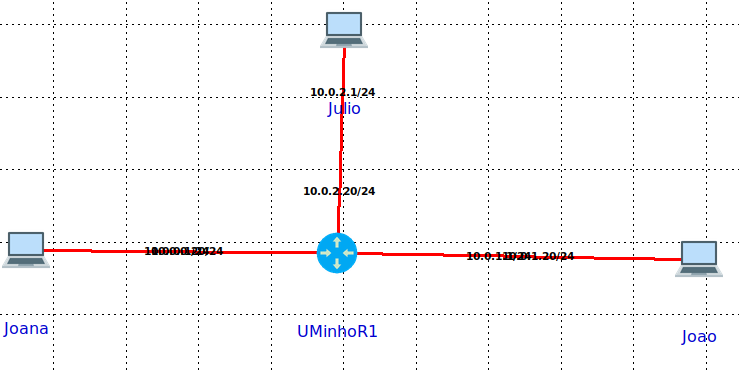
\includegraphics[width=0.6\textwidth]{imagens/tipologia.png}
    \caption{Topologia de rede implementada}
    \label{fig:tipologia_teste}
\end{figure}

\section{Testes para a validação do funcionamento do sniffer}

\subsection{Validação da correta análise do ICMP}
Para validar o correto funcionamento do sniffer na deteção e interpretação de pacotes ARP, foi realizado um teste no ambiente CORE, com base na topologia de rede apresentada anteriormente na Figura \ref{fig:tipologia_teste}. 

O objetivo foi observar a geração de mensagens ARP Request e ARP Reply durante a comunicação entre os hosts da rede.

O comando utilizado para gerar tráfego foi o seguinte:

\begin{verbatim}
ping -c 5 8.8.8.8
\end{verbatim}

Este comando envia cinco pacotes ICMP Echo Request para o servidor DNS público da Google (8.8.8.8), permitindo observar tanto os pedidos como as respetivas respostas (Echo Reply).

Durante a execução do teste, o sniffer foi colocado em funcionamento na interface de rede ativa, capturando todo o tráfego associado à comunicação ICMP. A análise dos resultados foi realizada de forma comparativa com o Wireshark, ferramenta de referência para inspeção de tráfego de rede.

\begin{figure}[H]
    \centering
    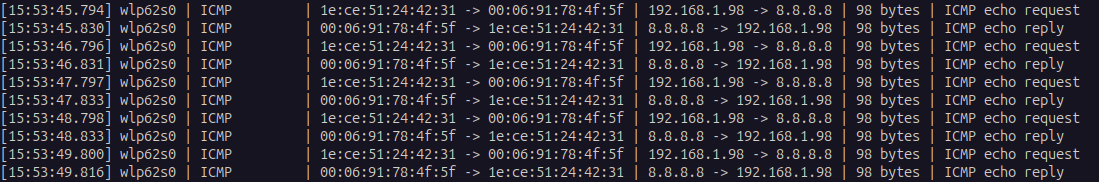
\includegraphics[width=1.05\linewidth]{imagens/ICMP_sniffer.png}
    \caption{Tráfego ICMP captado pelo nosso sniffer}
    \label{fig:icmp_sniffer}
\end{figure}

\begin{figure}[H]
    \centering
    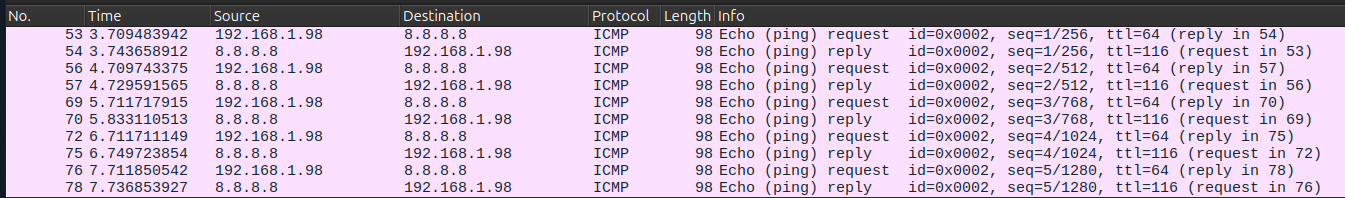
\includegraphics[width=1.05\linewidth]{imagens/ICMP_wireshark.png}
    \caption{Tráfego ICMP captado pelo Wireshark}
    \label{fig:icmp_wireshark}
\end{figure}


A análise comparativa entre o sniffer desenvolvido e o Wireshark permite concluir que a implementação se encontra corretamente funcional na deteção de tráfego ICMP. Observa-se que ambos os sistemas apresentam informação consistente relativamente aos pacotes capturados, nomeadamente na identificação do protocolo ICMP, nos endereços IP de origem e destino, na dimensão dos pacotes e na correspondência entre mensagens Echo Request e Echo Reply. 

Desta forma, podemos concluir que os resultados obtidos pelo sniffer estão em conformidade com os apresentados pelo Wireshark, confirmando a corretude da análise efetuada.

\subsection{Validação da correta análise do TCP}

Para validar o funcionamento do sniffer na deteção e interpretação de segmentos TCP, foi utilizado o ambiente CORE com a topologia de rede previamente apresentada na Figura \ref{fig:tipologia_teste}.

O objetivo deste teste foi observar o estabelecimento e encerramento de ligações TCP, permitindo confirmar a correta identificação do \textit{three-way handshake}, bem como das flags associadas à comunicação.

O tráfego foi gerado através da abertura de uma ligação TCP entre dois hosts da rede. Para tal, num terminal do host João foi executado:

\begin{verbatim}
nc -l -p 5000
\end{verbatim}

Num segundo terminal, no host Joana, foi executado:

\begin{verbatim}
echo "teste" | nc 10.0.1.20 5000
\end{verbatim}

Este procedimento força o estabelecimento de uma ligação TCP para a porta 5000, transmitindo dados e encerrando a sessão após a comunicação.

Durante a execução do teste, o sniffer permaneceu ativo na interface de rede em monitorização, capturando todos os segmentos TCP trocados. Em paralelo, o Wireshark foi utilizado como ferramenta de referência para validação dos resultados.

\begin{figure}[H]
    \centering
    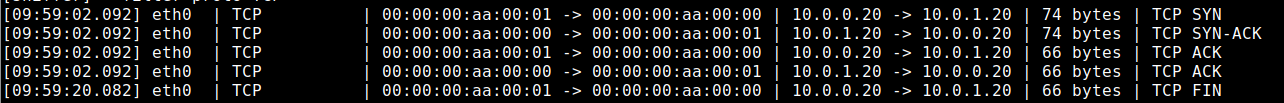
\includegraphics[width=1.05\linewidth]{imagens/tcp_sniffer.png}
    \caption{Tráfego TCP captado pelo nosso sniffer}
    \label{fig:tcp_sniffer}
\end{figure}

\begin{figure}[H]
    \centering
    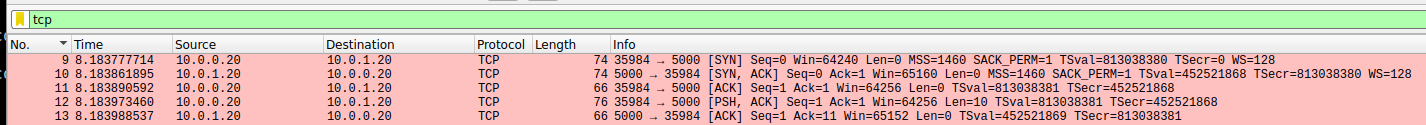
\includegraphics[width=1.05\linewidth]{imagens/tcp_wireshark.png}
    \caption{Tráfego TCP captado pelo Wireshark}
    \label{fig:tcp_wireshark}
\end{figure}

A análise comparativa entre a Figura \ref{fig:tcp_sniffer} e a Figura \ref{fig:tcp_wireshark} permite confirmar o correto funcionamento do módulo TCP implementado no sniffer.

Observa-se, em ambas as capturas, a sequência típica de estabelecimento de ligação TCP através do \textit{three-way handshake}, composta pelos segmentos \texttt{SYN}, \texttt{SYN-ACK} e \texttt{ACK}. O sniffer desenvolvido conseguiu identificar corretamente esta sequência, bem como os endereços IP de origem e destino envolvidos na comunicação entre os hosts \texttt{10.0.0.20} e \texttt{10.0.1.20}.

Após a fase inicial de ligação, o Wireshark apresenta um segmento adicional identificado como \texttt{PSH, ACK}, correspondente à transmissão efetiva de dados enviada pelo comando \texttt{echo "teste"}. No sniffer desenvolvido, este segmento surge classificado genericamente como \texttt{ACK}. Esta diferença deve-se ao facto de a implementação atual privilegiar a deteção das flags principais associadas ao estado da ligação, não distinguindo ainda combinações compostas como \texttt{PSH-ACK}. Ainda assim, o segmento foi corretamente capturado e contabilizado como tráfego TCP válido.

Relativamente ao encerramento da sessão, o sniffer identificou corretamente a flag \texttt{FIN}, demonstrando capacidade para reconhecer o término normal da ligação TCP. Este comportamento encontra-se igualmente de acordo com o fluxo esperado para este tipo de comunicação.

Desta forma, conclui-se que o sniffer desenvolvido se encontra corretamente funcional na análise de tráfego TCP, identificando os principais estados da ligação, reconhecendo o estabelecimento e encerramento de sessões e apresentando resultados consistentes com os observados no Wireshark.

\subsection{Validação da correta análise do ARP}

Para validar o funcionamento do sniffer na deteção e interpretação de pacotes ARP, utilizou-se a topologia montada no ambiente CORE. A rede é composta pelos hosts \texttt{Joana} (10.0.0.1), \texttt{Joao} (10.0.1.20) e \texttt{Julio}, ligados pelo router \texttt{UMinhoR1}, conforme ilustrado na Figura \ref{fig:tipologia_teste}.

O tráfego foi gerado a partir de um teste de conectividade, executando o seguinte comando no host \texttt{Joana}:

\begin{verbatim}
ping -c 5 10.0.1.20
\end{verbatim}

Durante a execução, o sniffer capturou o tráfego na interface \texttt{eth0}. Em paralelo, o Wireshark foi utilizado como ferramenta de referência para validação dos resultados.

\begin{figure}[H]
\centering
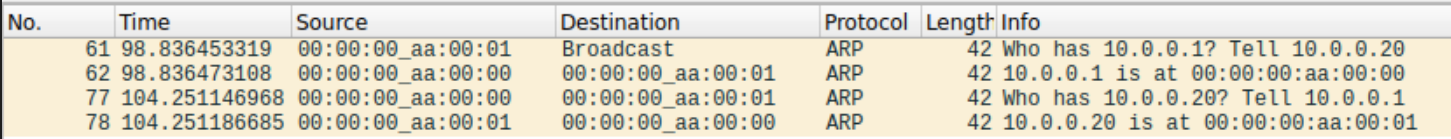
\includegraphics[width=1.05\linewidth]{imagens/arp_wireshark.png}
\caption{Tráfego ARP captado pelo Wireshark}
\label{fig:arp_wireshark}
\end{figure}

\begin{figure}[H]
\centering
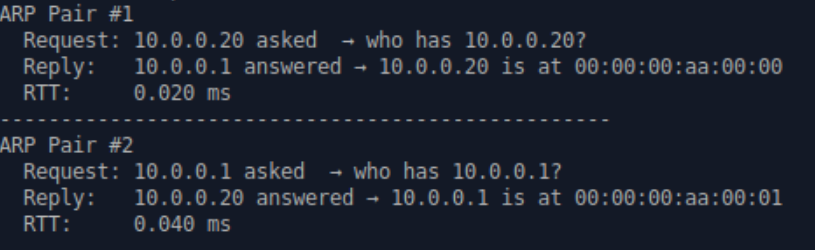
\includegraphics[width=0.8\linewidth]{imagens/arp_sniffer.png}
\caption{Saída do sniffer para os pares ARP identificados}
\label{fig:arp_sniffer}
\end{figure}

Na Figura \ref{fig:arp_wireshark} observa-se o tráfego ARP captado pelo Wireshark. Foram gerados dois pares completos de mensagens ARP. O primeiro par (pacotes 61 e 62) corresponde ao pedido para descobrir o endereço físico associado ao destino, seguido da respetiva resposta. O segundo par (pacotes 77 e 78) representa o processo de resolução inverso, permitindo que ambos os intervenientes atualizem as suas tabelas ARP.

Na Figura \ref{fig:arp_sniffer} apresenta-se a saída do sniffer desenvolvido. Os dois pares ARP foram identificados e relacionados com sucesso, sendo possível observar os endereços IP envolvidos, os respetivos endereços MAC e o RTT (\textit{Round-Trip Time}) calculado para cada par (0.020 ms e 0.040 ms, respetivamente).

Os valores de RTT obtidos correspondem ao intervalo entre o \textit{ARP Request} e o \textit{ARP Reply}, refletindo a latência de resolução de endereços na rede local simulada. É possível reparar que, apesar de terem sido enviados vários pacotes ICMP, apenas um número reduzido de mensagens ARP foi observado. Tal deve-se ao facto de as associações IP–MAC serem armazenadas em cache pelos hosts, evitando a redundância de pedidos após a resolução inicial.

Desta forma, conclui-se que o sniffer identifica os pacotes ARP, distingue entre pedidos e respostas, correlaciona os pares e calcula o RTT de forma adequada, apresentando resultados consistentes com os observados no Wireshark.


\subsection{Validação da correta análise do IPv4}

Para validar o funcionamento do sniffer na deteção e interpretação de pacotes IPv4,
utilizou-se a topologia montada no ambiente CORE, com base na configuração apresentada
anteriormente na Figura \ref{fig:tipologia_teste}.

O objetivo deste teste foi observar a fragmentação de pacotes IPv4, confirmando a correta
identificação dos campos do cabeçalho, nomeadamente o campo \texttt{ID}, o \textit{Fragment Offset}
e as flags \texttt{MF} e \texttt{DF}.

O tráfego foi gerado a partir do host \texttt{Joana} (10.0.0.20), executando o seguinte comando:

\begin{verbatim}
ping -c 1 -s 2000 10.0.0.1
\end{verbatim}

Este comando envia um pacote ICMP de 2000 bytes para o \texttt{UMinhoR1} (10.0.0.1), valor
superior ao MTU padrão de 1500 bytes, forçando assim a fragmentação ao nível IPv4.
Durante a execução, o sniffer capturou o tráfego na interface \texttt{eth0} do \texttt{UMinhoR1}.
Em paralelo, o Wireshark foi utilizado como ferramenta de referência para validação dos resultados.

\begin{figure}[H]
\centering
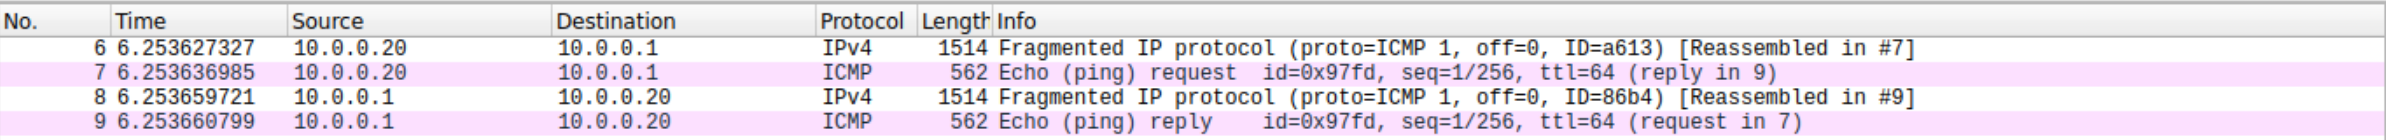
\includegraphics[width=1.05\linewidth]{imagens/ipv4_wireshark.png}
\caption{Tráfego IPv4 fragmentado captado pelo Wireshark}
\label{fig:ipv4_wireshark}
\end{figure}

\begin{figure}[H]
\centering
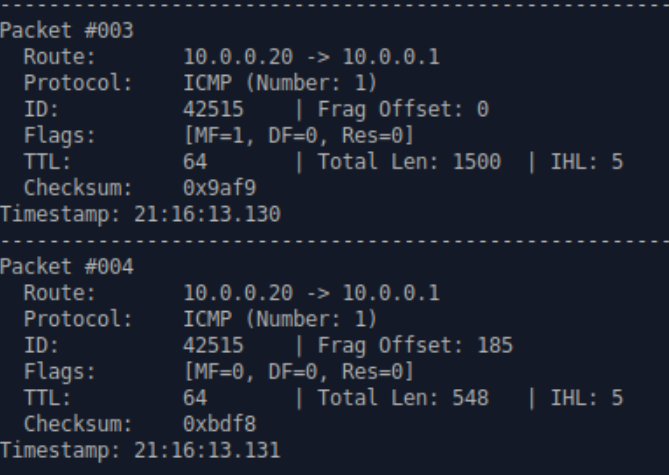
\includegraphics[width=0.7\linewidth]{imagens/ipv4_sniffer.png}
\caption{Saída do sniffer para os fragmentos IPv4 identificados}
\label{fig:ipv4_sniffer}
\end{figure}

Na Figura \ref{fig:ipv4_wireshark} observa-se o tráfego capturado pelo Wireshark. O pacote
ICMP de 2000 bytes foi dividido em dois fragmentos IPv4, ambos partilhando o mesmo
identificador (\texttt{ID=a613}). O primeiro fragmento (pacote 6) apresenta \texttt{MF=1} e offset 0,
indicando que existem mais fragmentos a seguir. O Wireshark indica a reassemblagem no
pacote 7, correspondente ao Echo Request ICMP completo. O mesmo processo ocorre no
sentido inverso, com a resposta do \texttt{UMinhoR1} para a \texttt{Joana} (pacotes 8 e 9).

Na Figura \ref{fig:ipv4_sniffer} apresenta-se a saída do sniffer desenvolvido. Os pacotes
\#003 e \#004 correspondem ao datagrama fragmentado com \texttt{ID=42515}, enviado por
\texttt{10.0.0.20} para \texttt{10.0.0.1}. O pacote \#003 apresenta \texttt{MF=1} e offset 0,
indicando que é o primeiro fragmento e que existem mais a seguir. O pacote \#004 apresenta
\texttt{MF=0} e offset 185 (equivalente a 1480 bytes), confirmando que se trata do fragmento
final. Ambos partilham o mesmo \texttt{ID} (42515), o mesmo \texttt{TTL} (64) e o mesmo protocolo
encapsulado (ICMP), o que permite a sua associação como pertencentes ao mesmo datagrama original.


A correspondência entre os dois datagramas pode ser confirmada através do campo \texttt{ID}: 
o Wireshark apresenta o valor em hexadecimal (\texttt{0xa613}), enquanto o sniffer apresenta 
o mesmo valor em decimal (\texttt{42515}), sendo ambos numericamente equivalentes 
(\texttt{0xa613} = \texttt{42515}).



Os resultados obtidos pelo sniffer são consistentes com os observados no Wireshark,
confirmando a correta identificação dos campos do cabeçalho IPv4, nomeadamente o
\texttt{ID}, o \textit{Fragment Offset}, as flags \texttt{MF} e \texttt{DF}, o \texttt{TTL} e o \textit{checksum}.
Conclui-se assim que o sniffer desenvolvido é capaz de capturar e analisar corretamente
pacotes IPv4, incluindo situações de fragmentação.



\subsection{Validação da correta análise IEEE 802.11 (WiFi)}

Para validar o correto funcionamento do módulo de análise de tráfego IEEE 802.11, foi realizada uma captura de pacotes em modo monitor utilizando uma interface wireless configurada para inspeção de frames ao nível da camada 2.

O objetivo deste teste foi verificar a capacidade do sistema em identificar corretamente os diferentes tipos de frames WiFi (Management, Control e Data), bem como a extração de informação relevante associada a redes e dispositivos observados no meio radioelétrico.

Durante a execução do teste, o sistema permaneceu ativo em modo de captura contínua, sendo observados frames IEEE 802.11 provenientes de múltiplos pontos de acesso e dispositivos na área envolvente. A geração de tráfego foi efetuada através da atividade normal de redes WiFi próximas, incluindo transmissão periódica de beacons, processos de associação de clientes e emissão de probe requests.

Os resultados obtidos foram agregados pelo sistema e encontram-se representados na Figura~\ref{fig:wifi_sniffer}.

\begin{figure}[H]
\centering
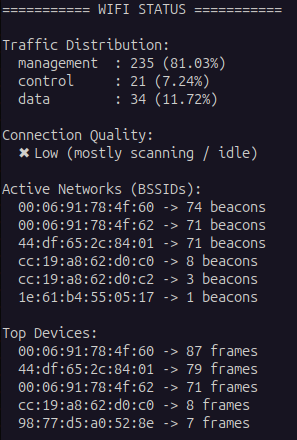
\includegraphics[width=0.35\linewidth]{imagens/wifi_status.png}
\caption{Resumo estatístico do tráfego IEEE 802.11 capturado pelo sniffer}
\label{fig:wifi_sniffer}
\end{figure}

\subsubsection{Análise dos resultados}

A análise dos resultados permite observar uma distribuição de tráfego dominada por frames de gestão (\textit{management frames}), representando aproximadamente 81\% do total capturado. Este comportamento é esperado em ambientes WiFi reais, uma vez que este tipo de frames inclui beacons, probe requests e mensagens de controlo da infraestrutura da rede.

Os frames de dados representam cerca de 11\% do total, refletindo a presença de tráfego de utilizador ativo nas redes detetadas. Já os frames de controlo apresentam uma percentagem reduzida, sendo consistentes com o seu papel auxiliar no acesso ao meio.

Adicionalmente, o sistema foi capaz de identificar múltiplos BSSIDs distintos, correspondentes a diferentes pontos de acesso IEEE 802.11 presentes no ambiente. Para cada BSSID, foi contabilizado o número de beacons recebidos, permitindo caracterizar a presença e atividade das redes sem fios.

No que diz respeito aos dispositivos ativos, o sistema registou múltiplos endereços MAC associados a diferentes níveis de atividade, refletindo a presença de clientes conectados ou em processo de descoberta de redes.

\subsubsection{Validação do sistema}

Os resultados obtidos demonstram a correta implementação do módulo de análise IEEE 802.11, evidenciando:

\begin{itemize}
    \item correta classificação dos frames em management, control e data;
    \item identificação consistente de redes através de BSSID;
    \item contabilização de beacons como indicador de presença de redes;
    \item deteção de dispositivos ativos através de endereços MAC;
    \item coerência global com o comportamento esperado de redes WiFi reais.
\end{itemize}

Desta forma, conclui-se que o sniffer desenvolvido é capaz de capturar, classificar e agregar corretamente tráfego IEEE 802.11 em tempo real, permitindo uma análise fiável do ambiente wireless envolvente.


\subsection{Validação da correta análise do DHCP}

Para validar o funcionamento do sniffer na deteção e interpretação de mensagens DHCP,
foi forçada uma renovação de endereço IP numa interface de rede real, através dos seguintes
comandos:

\begin{verbatim}
sudo dhcpcd -k eth0
sudo dhcpcd eth0
\end{verbatim}

Estes comandos libertam o endereço IP atual e iniciam um novo processo de negociação DHCP
com o servidor real da rede, gerando a sequência completa de mensagens DORA
(\textit{Discover, Offer, Request, ACK}). Durante a execução, o sniffer e o Wireshark
foram colocados em funcionamento simultaneamente na interface \texttt{eth0}, permitindo
a comparação direta dos resultados.


\begin{figure}[H]
\centering
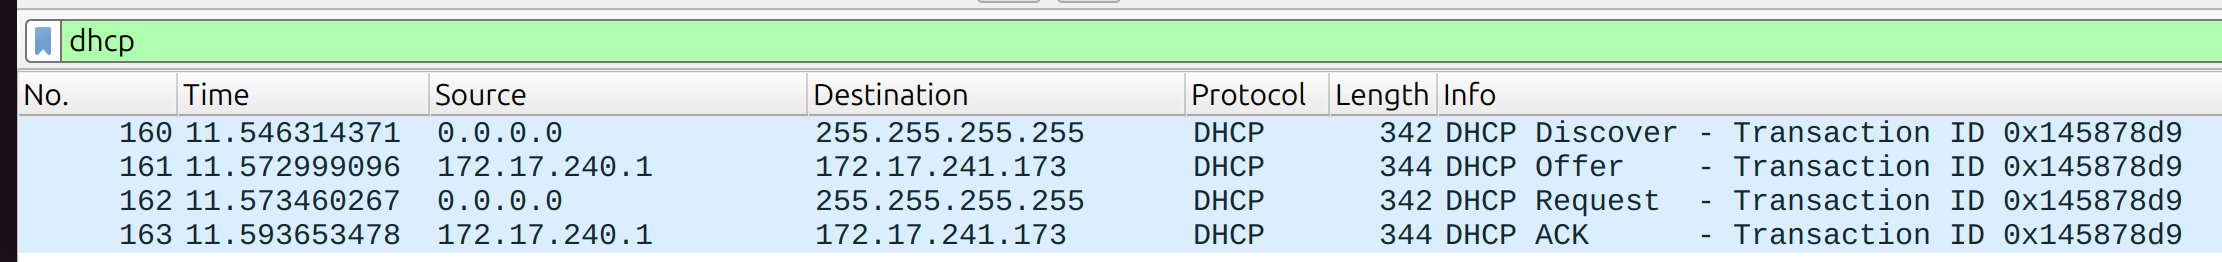
\includegraphics[width=1.05\linewidth]{imagens/dhcp_wireshark.png}
\caption{Tráfego DHCP captado pelo Wireshark}
\label{fig:dhcp_wireshark}
\end{figure}

\begin{figure}[H]
\centering
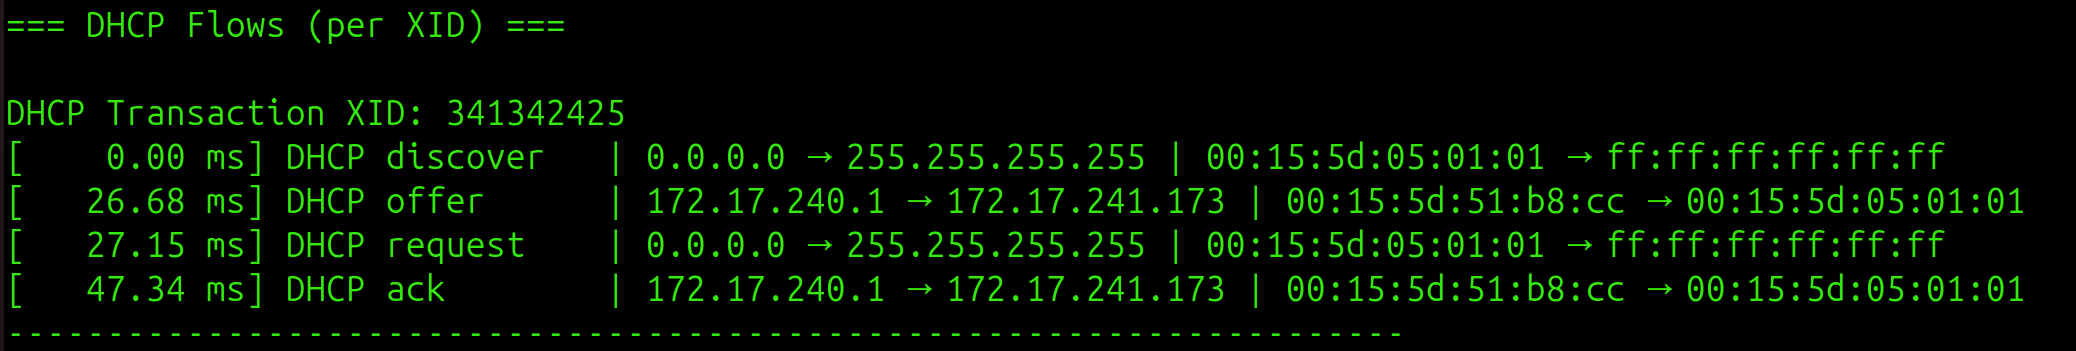
\includegraphics[width=1.05\linewidth]{imagens/dhcp_sniffer.png}
\caption{Tráfego DHCP captado pelo sniffer}
\label{fig:dhcp_sniffer}
\end{figure}

Na Figura \ref{fig:dhcp_wireshark} observa-se a sequência DORA completa capturada pelo
Wireshark. O processo inicia-se com um \textit{DHCP Discover} enviado em broadcast
(\texttt{0.0.0.0 → 255.255.255.255}), ao qual o servidor responde com um \textit{DHCP Offer}
contendo o endereço proposto (\texttt{172.17.241.173}). O host confirma com um
\textit{DHCP Request} e o servidor finaliza com um \textit{DHCP ACK}. Todas as mensagens
partilham o mesmo \textit{Transaction ID} \texttt{0x145878d9}.

Na Figura \ref{fig:dhcp_sniffer} apresenta-se o output do sniffer desenvolvido. A transação
foi corretamente identificada e agrupada pelo \textit{XID} \texttt{341342425}. Este valor
corresponde ao \textit{Transaction ID} \texttt{0x145878d9} apresentado pelo Wireshark,
sendo numericamente equivalentes — o Wireshark apresenta o valor em hexadecimal enquanto
o sniffer o apresenta em decimal (\texttt{0x145878d9} = \texttt{341342425}). Esta
correspondência confirma que ambas as ferramentas identificaram a mesma transação DHCP.
O sniffer apresenta ainda os tempos relativos de cada mensagem em relação ao \textit{Discover},
permitindo observar que o processo de negociação completo demorou aproximadamente 47 ms.

Os resultados obtidos pelo sniffer são consistentes com os observados no Wireshark,
confirmando a correta identificação e agrupamento das mensagens DHCP, bem como o
cálculo dos tempos relativos de cada fase da negociação.
Conclui-se assim que o sniffer desenvolvido é capaz de capturar e analisar corretamente
o protocolo DHCP, identificando a sequência DORA e associando corretamente as mensagens
pertencentes à mesma transação.

\section{Análise em Interface de Rede Real}

Para complementar os testes realizados no ambiente controlado (CORE), o sniffer foi também executado numa interface de rede real, permitindo observar o comportamento do tráfego em condições reais.

A captura foi realizada numa interface ativa (ex.: \texttt{wlan0}), em modo contínuo, durante a utilização normal da rede (navegação web, acesso a serviços online, etc.).

\subsection{Observações}

Durante a captura, foi possível identificar diversos tipos de tráfego, nomeadamente:

\begin{itemize}
    \item Tráfego \textbf{TCP}, associado a ligações HTTP/HTTPS, com múltiplos handshakes e trocas de dados;
    \item Pacotes \textbf{ICMP}, utilizados em testes de conectividade e controlo de rede;
    \item Mensagens \textbf{ARP}, resultantes da resolução de endereços na rede local;
    \item Tráfego \textbf{DHCP}, observado em momentos de renovação de endereço IP;
    \item Frames \textbf{IEEE 802.11}, evidenciando atividade de redes WiFi próximas.
\end{itemize}

Verificou-se que o volume de tráfego em ambiente real é significativamente superior ao ambiente simulado, com múltiplas comunicações concorrentes e maior diversidade de protocolos.

\subsection{Resultados}

O sniffer demonstrou capacidade para:

\begin{itemize}
    \item Capturar pacotes em tempo real sem perdas significativas;
    \item Identificar corretamente os protocolos presentes;
    \item Aplicar os handlers implementados em cenários reais;
    \item Produzir estatísticas consistentes com o comportamento observado.
\end{itemize}

Estes resultados confirmam a aplicabilidade da ferramenta em ambientes reais, para além do contexto académico e simulado.

\section{Obstáculos Encontrados}

Durante o desenvolvimento do sniffer, foram encontrados diversos desafios técnicos, tanto ao nível da captura como da análise dos pacotes:

\begin{itemize}

\item \textbf{Identificação do protocolo principal (top\_protocol)}  
A determinação do protocolo principal de cada pacote revelou-se não trivial, uma vez que um único pacote pode conter múltiplas camadas (por exemplo, IPv4 + ICMP ou IPv4 + TCP).  
Foi necessário definir uma lógica consistente que permitisse identificar corretamente o protocolo dominante, garantindo simultaneamente que os handlers apropriados eram invocados (por exemplo, processar um pacote tanto no handler IPv4 como no handler ICMP).

\item \textbf{Captura em ambiente real com elevado volume de tráfego}  
A transição do ambiente simulado (CORE) para uma interface real introduziu um volume significativamente superior de pacotes, com múltiplas comunicações simultâneas.  
Este cenário exigiu maior eficiência no processamento, levando à introdução de um modo com menor verbosidade, que reduz o overhead associado à formatação e output dos pacotes, melhorando assim o desempenho em cenários de elevado volume de tráfego.

\item \textbf{Captura de pacotes em modo monitor}  
A configuração de interfaces WiFi em modo monitor revelou-se dependente do sistema operativo e drivers, dificultando a captura de frames IEEE 802.11.

\item \textbf{Reconstrução e correlação de fluxos}  
A associação entre pacotes relacionados (ex.: pedidos e respostas em ICMP e ARP, ou fases do handshake TCP) exigiu a definição de chaves únicas e tratamento de situações em que pacotes podem chegar fora de ordem ou não serem capturados.

\item \textbf{Gestão de fragmentação IPv4}  
A identificação e agrupamento correto de fragmentos implicou compreender detalhadamente os campos do cabeçalho IP (ID, offset, flags).

\item \textbf{Interpretação de protocolos complexos}  
Protocolos como DHCP e TCP exigem análise de múltiplos estados, tornando a implementação mais complexa do que protocolos simples como ARP.

\end{itemize}

\section{Limitações da Aplicação Desenvolvida}

Apesar dos resultados obtidos, o sniffer apresenta algumas limitações:

\begin{itemize}

\item \textbf{Análise parcial de flags TCP}  
A implementação não distingue todas as combinações de flags (ex.: PSH-ACK), tratando apenas os estados principais.

\item \textbf{Dependência da biblioteca Scapy}  
A análise dos pacotes depende das funcionalidades disponibilizadas pela biblioteca Scapy, podendo existir limitações na dissecação de certos protocolos ou campos específicos.

\item \textbf{Limitações na captura de tráfego WiFi}  
A captura de frames IEEE 802.11 depende do suporte da interface de rede para modo monitor, o que nem sempre está disponível ou corretamente configurado.

\item \textbf{Escalabilidade e uso de memória}  
A utilização de estruturas em memória para armazenar pacotes e dados de análise pode tornar-se ineficiente em capturas de longa duração ou com elevado volume de tráfego.

\item \textbf{Ausência de interface gráfica}  
O sistema funciona exclusivamente em linha de comandos, o que limita a visualização e exploração interativa dos dados quando comparado com ferramentas como o Wireshark.

\item \textbf{Análise limitada a protocolos implementados}  
A aplicação apenas suporta análise detalhada dos protocolos para os quais existem handlers implementados, não sendo extensível automaticamente a novos protocolos.

\end{itemize}

\section{Conclusão do Trabalho Efetuado}

O presente trabalho permitiu o desenvolvimento de um \textit{packet sniffer} funcional, capaz de capturar, analisar e interpretar tráfego de rede em múltiplos protocolos da pilha TCP/IP, bem como de redes sem fios IEEE 802.11.

A arquitetura modular adotada revelou-se fundamental para a organização do sistema, permitindo separar claramente as responsabilidades entre captura, parsing, análise por protocolo, estatísticas e apresentação de resultados. Esta abordagem facilitou a extensibilidade do projeto e a integração de novos módulos de forma consistente.

Ao longo do desenvolvimento, foram implementados handlers específicos para protocolos como ICMP, TCP, ARP, DHCP, IPv4 e WiFi, permitindo não apenas a identificação dos pacotes, mas também a reconstrução de interações relevantes, como o \textit{three-way handshake} TCP, a sequência DORA do DHCP ou o emparelhamento request/reply em ICMP e ARP.

Os testes realizados em ambiente controlado (CORE) e em interface de rede real permitiram validar o correto funcionamento do sistema, demonstrando a sua capacidade de operar em diferentes cenários e sob diferentes volumes de tráfego. A comparação com ferramentas de referência, como o Wireshark, confirmou a consistência dos resultados obtidos.

Apesar dos resultados positivos, foram identificadas algumas limitações, nomeadamente ao nível da profundidade da análise de certos protocolos, da escalabilidade em ambientes de elevado tráfego e da ausência de uma interface gráfica.

Em conclusão, o trabalho cumpriu os objetivos propostos, fornecendo uma ferramenta funcional para análise de tráfego de rede e contribuindo para uma melhor compreensão do funcionamento dos principais protocolos das camadas de rede, transporte e aplicação.

\end{document}